\let\negmedspace\undefined
\let\negthickspace\undefined
\documentclass[journal,12pt,twocolumn]{IEEEtran}
\usepackage{cite}
\usepackage{amsmath,amssymb,amsfonts,amsthm}
\usepackage{algorithmic}
\usepackage{graphicx}
\usepackage{textcomp}
\usepackage{xcolor}
\usepackage{txfonts}
\usepackage{listings}
\usepackage{enumitem}
\usepackage{mathtools}
\usepackage{gensymb}
\usepackage{comment}
\usepackage[breaklinks=true]{hyperref}
\usepackage{tkz-euclide}
\usepackage{listings}
\usepackage{gvv}
\def\inputGnumericTable{}
\usepackage[latin1]{inputenc}
\usepackage{color}
\usepackage{array}
\usepackage{longtable}
\usepackage{calc}
\usepackage{multirow}
\usepackage{hhline}
\usepackage{ifthen}
\usepackage{lscape}

\newtheorem{theorem}{Theorem}[section]
\newtheorem{problem}{Problem}
\newtheorem{proposition}{Proposition}[section]
\newtheorem{lemma}{Lemma}[section]
\newtheorem{corollary}[theorem]{Corollary}
\newtheorem{example}{Example}[section]
\newtheorem{definition}[problem]{Definition}
\newcommand{\BEQA}{\begin{eqnarray}}
\newcommand{\EEQA}{\end{eqnarray}}
\newcommand{\define}{\stackrel{\triangle}{=}}
\theoremstyle{remark}
\newtheorem{rem}{Remark}
\begin{document}

\bibliographystyle{IEEEtran}
\vspace{3cm}

\title{Gate 2023- Instrumentation Engineering}
\author{EE23BTECH11058 - Sindam Ananya$^{*}$% <-this % stops a space
}
\maketitle
\newpage
\bigskip

\renewcommand{\thefigure}{\theenumi}
\renewcommand{\thetable}{\theenumi}

\vspace{3cm}
\textbf{Question 60:} 
In the circuit shown, the input voltage $V_{in} = 100mV$. The switch and the opamp are ideal. At time $t=0$, the intial charge stored in the $10nF$ capacitor is $1nC$, with the polarity as indicated in the figure. The switch $S$ is controlled using a $1KHz$ square-wave voltage signal $V_s$ as shown. Whenever $V_s$ is `High', $S$ is in position $`1$' and when $V_s$ is `Low', $S$ is in position `$2$'.\\
At $t = 20ms$, the magnitude of the voltage $V_o$ will be  \\  
\begin{figure}[h!]
    \centering
    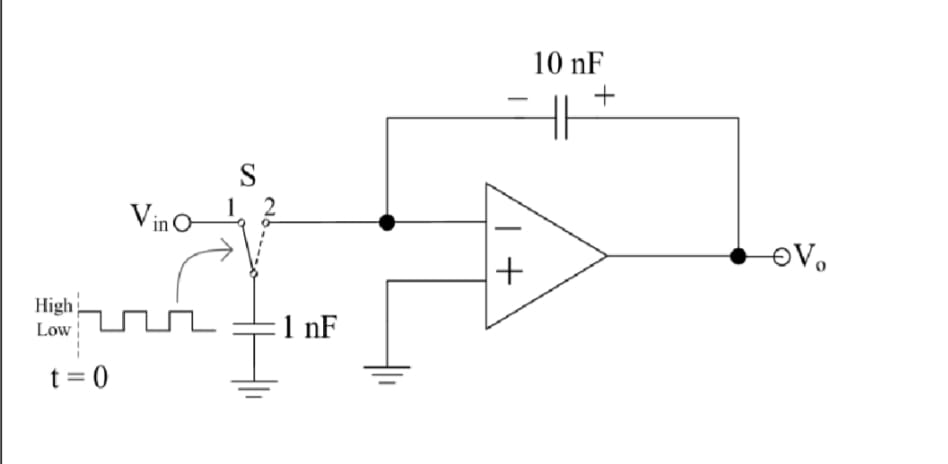
\includegraphics[width=\columnwidth]{figs/ingate60.png}
    \label{fig:ingate60}
\end{figure}
\hfill{(GATE ST 2023)}\\
\solution
\begin{table}[h!]
    \centering
    \begin{tabular}{|c|c|c|}
        \hline
        \textbf{Parameter} & \textbf{Value} & \textbf{Description} \\
        \hline
        $V_{in}$ & $100mV$ & Input voltage \\
        \hline
        $q_{10nF}$ & $1nC$ & Intial charge on $10nF$ \\
        \hline
        $f$ & $1KHz$ & Frequency of $V_s$ \\
        \hline
        $V_o$ &  & Output voltage \\
        \hline
    \end{tabular}

    \caption{Input Parameters}
    \label{tab:gatein60table}
\end{table}
$ 0 < t < 0.5ms $
\begin{align}
q_{1nF} &= 100mV \times 1nF\\ 
        &= 0.1nC
\end{align}
$ 0.5ms < t < 1ms $\\
Both the capcitors will discharge
\begin{align}
q_{10nF} &= 1nC - 0.1nC\\
         &= 0.9nC
\end{align}
At $t = 20ms$,
\begin{align}
q_{10nF} &= 1nC - 20 \brak{0.1nC}\\
         &= -1nC\\
V_o &= \frac{-1nC}{10nF}\\
    &= -100mV
\end{align}
\end{document}
